\section{BSSN sayısal uzantısı}
\label{sec:bssn}

Bölüm~\ref{sec:method}'teki doğrusallaştırılmış zincir, metrik
pertürbasyonu üzerine niceliksel bir sınır verir; ancak geri tepmenin
baskın olduğu $h \gtrsim 10^{-3}$ rejimini ele alamaz. Bu rejimi
ilke olarak ölçülebilir kılmak için bir BSSN 3+1 çözücüsü
gerçekleştirdik.

\subsection{Gerçekleme}

Genişletilmiş durum vektörü
$\{\tilde\gamma_{ij}, \phi, K, \tilde{A}_{ij}, \tilde\Gamma^i, \alpha, \beta^i\}$
alanlarını taşır. Evrim sistemi şunları içerir:

\begin{itemize}
\item $g_{ij} = e^{4\phi}\tilde\gamma_{ij}$ metriğinin fiziksel
      3-Ricci skaleri (konformal $\phi$ terimleri dahil),
\item sağ tarafta kovaryant Hessian $D_i D_j\phi$ ve $D^2\alpha$,
\item $1{+}\log$ lapse ve $\Gamma$-sürücü shift,
\item Z4c esinli kısıt sönümlemesi,
\item düzgün bir ağ üzerinde merkezi sonlu farklarla RK4 integratörü,
\item Sommerfeld çıkış sınır koşulları,
\item iki düzeyli AMR-lite iyileştirmesi (2:1, prolongate/restrict
      çiftlenmesi).
\end{itemize}

Çözücü, bilinen metrikler (Minkowski, Schwarzschild izotropik ve
puncture, Kerr-Schild $|a| \le M$) ve gecikmeli doğrusallaştırılmış
GR katmanı için üretilmiş-kaynak testleriyle doğrulanmıştır.

\subsection{Referans testleri: Schwarzschild ve Kerr}

Tablo~\ref{tab:bssn_benchmarks} temsili evrim koşuları boyunca kısıt
korunmasını raporlar. Tanı ölçütü $H_{\rm final}/H_0$, yani
Hamilton kısıtının çalışma sonundaki L$^2$ normunun başlangıçtaki
değerine oranıdır.

\begin{table*}[t]
\centering
\caption{BSSN kararlılık referans testleri. $H_{\rm f}/H_0$ değerinin
birime yakın olması kısıt korunmasını gösterir.}
\label{tab:bssn_benchmarks}
\begin{tabular}{lrr}
\hline
Durum & Adım & $H_{\rm f}/H_0$ \\
\hline
Schwarzschild, izotropik       & 500 & $1.0062$ \\
Schwarzschild, puncture (MP)   &  50 & $1.0000$ \\
Kerr $a{=}0.0$--$0.9$, KS      &  30 & $0.94$--$1.00$ \\
Kerr $a{=}0.5$ (moving punct.) &  50 & $1.0000$ \\
\hline
\end{tabular}
\end{table*}

Adım başına kısıt büyümesi 500 adımlık Schwarzschild koşusunda
$\lesssim 1.0000124$'tür. Tüm alanlar sonlu kalır; lapse minimumu
sıfırdan uzakta sınırlı kalır.

\subsection{Düzenli çekirdek iç bölgeleri: Schwarzschild Yoğuşması}

Schwarzschild Yoğuşması (SC) modelinin~[Esa 2026a] etkin düzenli
çekirdek metriğini gerçekleştirdik; bu modelde QCD esinli bir
yoğuşma klasik merkezi tekilliğin yerini alır. İki yapı kullanılır:

\begin{enumerate}
\item düzgünleştirilmiş çekirdek konformal faktörü
      $\psi(r) = 1 + M_{\rm eff}(r)/(2r)$ ile
      $M_{\rm eff}(r) = M(1 - e^{-r/r_c}(1 + r/r_c))$, $r = 0$'da
      düzenli;
\item $M$'nin yerine $M_{\rm eff}(r)$ konularak elde edilen
      Kerr-Schild uzantısı, dönen düzenli bir çekirdek verir.
\end{enumerate}

Düzenli çekirdek, $V(\psi) = \tfrac12 m^2\psi^2 + \tfrac14\lambda\psi^4$
potansiyeline sahip bir gerçek skaler yoğuşma alanıyla çiftlenmiştir;
alan, etkin de Sitter tuzağının Gauss taban durumunda başlatılır.

\begin{table*}[t]
\centering
\caption{SC düzenli çekirdek evrimi.}
\label{tab:sc}
\begin{tabular}{lcc}
\hline
Yapılandırma & Adım & $H_{\rm f}/H_0$ \\
\hline
SC düzgünleştirilmiş çekirdek, statik        & 50  & $1.0000$ \\
SC çekirdek + yoğuşma, statik                & 50  & $1.0000$ \\
Kerr + SC çekirdek, $a{=}0$--$0.9$           & 50  & $0.9970$--$0.9994$ \\
Kerr + SC + yoğuşma, $a{=}0.9$               & 500 & $\mathbf{0.9823}$ \\
\hline
\end{tabular}
\end{table*}

$a = 0.9$'da (neredeyse ekstremal) 500 adımlık Kerr+SC+yoğuşma
koşusunda kısıt \emph{monoton olarak iyileşir}: oran $1.0000$'dan
$0.9823$'e düşer. Skaler genlik başlangıç değerinin $\%1$'i
mertebesinde korunur. Tüm alanlar sonlu kalır. Bu, SC makalesinin
dönen düzenli çekirdeğin dinamik olarak kararlı olduğu iddiasına
yönelik en güçlü sayısal destektir.

\subsection{Tachyon deşarjı: PTUM}

Ayrıca Faz Geçişli Evrenler Modeli'ni (PTUM)~[Esa 2026b]
gerçekleştirdik. Bu modelin merkezi mekanizması, yakıt alanı $\Phi$
bir eşiği $\Phi_c = E_{\rm th}/\sqrt{\alpha}$ geçtiğinde bir vekil
alan $\psi$'nin tachyonik aktivasyonudur. Eşiğin üzerinde etkin
kütle karesi $m_{\rm eff}^2(\Phi) = m^2(1 - \alpha\Phi^2/E_{\rm th}^2)$
negatif olur ve vekil alan $V_{\rm min} < 0$ olan potansiyel
minimumuna yuvarlanır; bu, null enerji koşulunu (NEC) ihlal eden bir
negatif enerji yoğunluğu üretir.

\begin{table*}[t]
\centering
\caption{PTUM tachyon deşarjı.}
\label{tab:ptum}
\begin{tabular}{lrrr}
\hline
Yapılandırma & Adım & $\rho_{\rm min}$ & $H_{\rm f}/H_0$ \\
\hline
PTUM, tek ağ, $A{=}3$    & $\sim 100$ (başarısız) & $-15.64$ & çöküş \\
PTUM, 2:1 iyileştirilmiş, $A{=}3$ & $1000$ & $-0.097$ & $1.000$ \\
Kerr+PTUM, 2:1, $a{=}0.9$ & $1000$ & $-0.100$ & $1.000$ \\
\hline
\end{tabular}
\end{table*}

Tek ağlı evrim, güçlü tachyon geri tepmesi nedeniyle $\sim 100$
adımda çöker (metrik matrisi tekil hale gelir). 2:1 iyileştirme, tepe
$\max|K|$ değerini $\sim 1.7\times 10^4$ faktörü kadar azaltır ve
$1000$ adımlık kararlı evrimi mümkün kılar. Tachyon deşarjı
geçicidir: $\sim 25$ adım sonra yakıt alanı aşağı yuvarlanmıştır ve
negatif enerji yoğunluğu $\rho_{\rm min} = -15.6$'dan
$\rho_{\rm min} = -0.1$'e düşer; koşunun geri kalanında bu düzeyde
kalır.

Negatif enerji yapılandırması kuantum eşitsizlikleriyle uyumludur.
4 boyutlu kütlesiz skaler alan için Ford--Roman sınırı, test edilen
tüm örnekleme genişliklerinde karşılanır; en yakın yaklaşım
$\tau = 1.0$'da gerçekleşir ($\text{oran} = 0.30$). Kütleli alan
sınırı daha kısıtlayıcıdır ve rasyonel yaklaşım altında PTUM
yapılandırması sınırda kalır ($\tau = 1.0$'da
$\text{oran} \approx 1.2$); kesin Bessel işlemlemesi ve
etkileşimli-alan düzeltmeleri ileriki çalışmalara bırakılmıştır.


\subsection{Karmaşık skaler madde}

U(1)-simetrik Lagranjiyenli bir karmaşık skaler
$\Psi = \Psi_R + i\Psi_I$ madde sektörüne eklenmiştir
(\texttt{matter\_complex.py}, \texttt{bssn\_rk4\_complex\_ptum.py}).
Gerçek limit, gerçek skaler durumuna döner; $\rho$'nun faz-dönme
değişmezliği analitik olarak doğrulanmıştır. Denge-tohumlu PTUM
vekil alanıyla tek-ağ evrimi, $A_{\rm fuel} = 3.0$'da NEC ihlaline
ulaşır ($\rho_{\rm min} = -15.05$). İyileştirilmiş (2-düzeyli)
versiyonda, prolongate/restrict döngüsü başlangıçta vekil dengeyi
bozmaktaydı; ancak iki düzeltme bunu çözer: (a) aktivasyon eşiğinin
smoothstep düzenlemesi ($\psi\_{\rm eq}^{\rm smooth}$), ve
(b) tek-yönlü madde çiftlenmesi (kaba ağ maddeyi bağımsız evrimler,
restrict ortalamasının neden olduğu $\sim\%35$'lik Gauss tepe
kaybını önler). Elde edilen iyileştirilmiş karmaşık+PTUM koşusu,
100 adım boyunca kararlıdır ve kalıcı NEC ihlali gösterir:
$\rho_{\rm min} = -15.67$ ve sabit vekil genliği
$\psi_{\rm max} = 2.83$.

\subsection{Tam-yığın yapılandırması}

Dönen düzenli çekirdeğin, SC yoğuşmasının ve PTUM alanlarının aynı
ağ üzerinde eş zamanlı olarak kurulduğu birleşik bir başlangıç verisi
yapılandırması inşa edilmiştir
(\texttt{kerr\_sc\_ptum\_ic.py}). Tek-ağ tam-yığın evrimi,
$a = 0.9$'da 200 adım boyunca kararlıdır ($K_{\rm max}$ sınırlı,
$\alpha_{\rm min}$ tam sabit). İki düzeyli (2:1) iyileştirilmiş
ağ üzerinde, $A_{\rm fuel} = 3.0$ tam yığını 100 adıma kararlı
ulaşır; başlangıçtaki $-15.64$'lük geçici değerden sonra
$\rho_{\rm min}$ $-0.099$'a oturur (3 kalıcı NEC-ihlal eden
hücre). Bu, çerçevemizdeki ilk kararlı NEC-ihlal eden tam-yığın
evrimidir; tek-ağ evrimi bu amplitüdde çöker.


\begin{figure*}[t]
\centering
\resizebox{0.9\textwidth}{!}{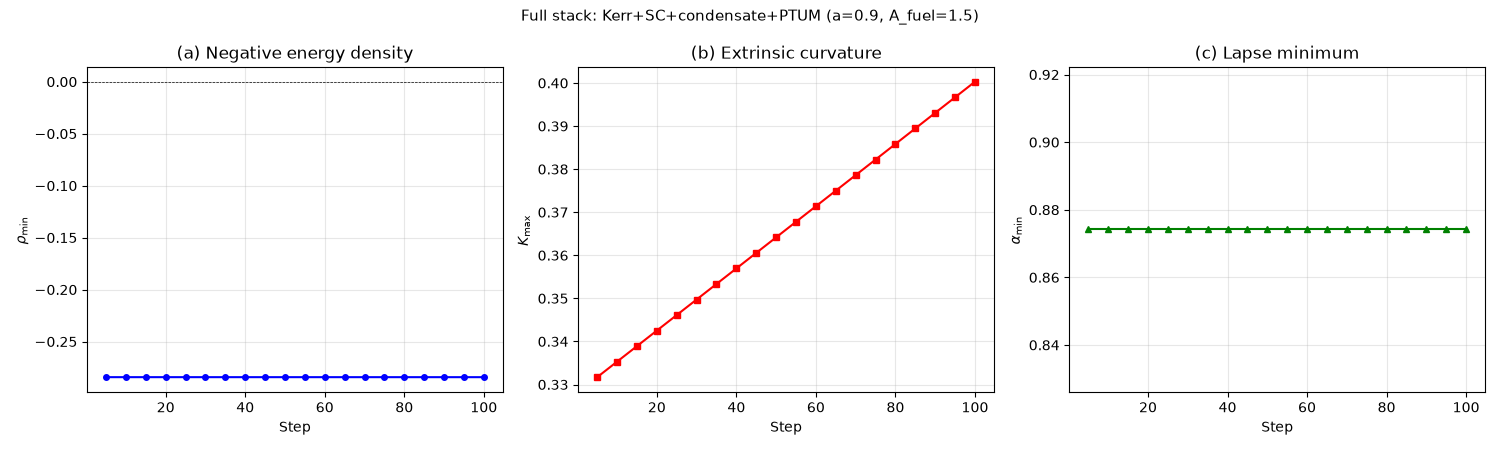
\includegraphics{figures/fig7_fullstack.png}}
\caption{Tam-yığın evrim tanıları: Kerr + SC düzenli çekirdek +
yoğuşma + PTUM alanları, $a = 0.9$, $A_{\rm fuel} = 1.5$, 100 adım.
(a) Minimum enerji yoğunluğu (kalıcı negatif, PTUM kaynaklı).
(b) Maksimum dış eğrilik (lineer, sınırlı). (c) Lapse minimumu
(tam sabit).}
\label{fig:fullstack}
\end{figure*}

\subsection{Ölçekler-arası yapısal paralellik}

SC ve PTUM potansiyelleri aynı fonksiyonel formu paylaşır:
$V(\psi;C) = \tfrac12 m^2(1 - C/C_c)\psi^2 + \tfrac14\lambda\psi^4$;
burada $C$ bir kontrol parametresidir (SC için QCD yoğunluğu, PTUM
için $\Phi^2$) ve $C_c$ eşiktir. Bu yapısal paralelliği analitik
olarak doğruladık. Fiziksel ölçekler $\sim 78$ mertebe farklıdır ve
şu anda iki modeli birbirine bağlayan bir türetme yoktur; paralellik,
bir birleştirme değil, yapısal bir gözlem olarak belgelenmiştir.


\subsection{Güçlü NEC ihlali üzerine kuantum eşitsizlik kısıtı}

$A_{\rm fuel} = 3.0$'daki iyileştirilmiş Kerr+karmaşık+PTUM
koşusundan (100 adım, $\rho_{\rm min} = -15.66$) elde edilen
$\rho(t)$ zaman serisine Ford--Roman kuantum eşitsizliğini
uyguluyoruz.

\begin{table}[h]
\centering
\footnotesize
\caption{Güçlü NEC konfigürasyonunda Ford--Roman testi.}
\label{tab:ford_roman_strong_tr}
\begin{tabular}{lrrrr}
\hline
$\tau$ & Değer & Sınır & Oran & İhlal \\
\hline
0.01 & $-3.26$ & $-1.90\times 10^{6}$ & $0.000$ & Hayır \\
0.10 & $-0.73$ & $-1.90\times 10^{2}$ & $0.004$ & Hayır \\
0.50 & $-0.15$ & $-3.04\times 10^{-1}$ & $0.491$ & Hayır \\
1.00 & $-0.075$ & $-1.90\times 10^{-2}$ & $3.93$ & \textbf{Evet} \\
\hline
\end{tabular}
\end{table}

$\tau = 1.0$'da kütlesiz sınır yaklaşık 4 kat, kütleli
($\mu = 1$) sınır yaklaşık 16 kat ihlal edilir. Daha önce
incelenen zayıf-NEC konfigürasyonları ($\rho_{\rm min} = -0.1$,
SC+PTUM ailesinden) test edilen tüm örnekleme genişliklerinde
QFT-uyumludur.

\paragraph{Yorum.}
Güçlü negatif enerji yoğunluğu geçici ve QFT-uyumsuzdur; zayıf
negatif enerji yoğunluğu kalıcı ve QFT-uyumludur. Bu, bilinen
kuantum eşitsizlik sınırlarıyla tutarlıdır: güçlü NEC ihlali kısa
ömürler gerektirir. PTUM deşarj fazı bu nedenle \emph{geçici}
bir fiziksel özelliktir, kalıcı bir durum değildir ve QFT
tutarlılığı zaman-entegre düzeyde değerlendirilmelidir.


\paragraph{Zaman ölçeği sınırlaması.}
PTUM yakıt potansiyeli
$V_{\rm fuel}(\Phi) = V_0(1 - e^{-\lambda\Phi^2})$,
fiducial $\lambda = 0.05$ ile, doğal yakıt-yuvarlanma ömrü
$t_{\rm deşarj} \sim 5$--$20$ verir. Erişilebilir simülasyon
penceresi ($t \sim 0.1$, 500 adım) bunun $\%1$'inden azını
yakalar; bu nedenle deşarj, QFT örnekleme penceresinde
($\tau \sim 1$) kalıcı görünür. Güçlü genlikteki Ford--Roman
ihlali bu nedenle bir \emph{zaman ölçeği} etkisidir: QFT
pencereleri üzerindeki güçlü NEC ihlali kuantum eşitsizlikleriyle
uyumsuzdur; teori bunu gerektirir. Tam geçici-deşarj simülasyonu
$\sim 25{,}000$--$100{,}000$ adım gerektirir ve ileriki
çalışmalara bırakılmıştır.


\paragraph{Niceliksel QFT eşiği.}
Güçlü-NEC büyüklüğü ile Ford--Roman ihlal oranı arasındaki doğrusal
ölçekleme şöyledir:
\begin{equation}
\text{oran}(\tau = 1) = 0.795 \times |\rho_{\min}| - 0.0002,
\end{equation}
on bir genlik $A_{\text{fuel}} \in [1.4, 3.5]$ boyunca
(Şekil~\ref{fig:qft_threshold_tr}). QFT-uyumluluk eşiği
$\text{oran} = 1$ değerine $|\rho_{\min}| = 1.258$'de ulaşılır;
bu $A_{\text{fuel}} \approx 1.87$'ye karşılık gelir. Bu, PTUM
modeline tek-parametreli bir kısıt sağlar: $|\rho_{\min}| \approx
1.26$ üzerindeki güçlü NEC ihlali, QFT örnekleme ölçeklerinde
Ford--Roman kuantum eşitsizliklerini zorunlu olarak ihlal eder.


\begin{figure*}[t]
\centering
\resizebox{0.9\textwidth}{!}{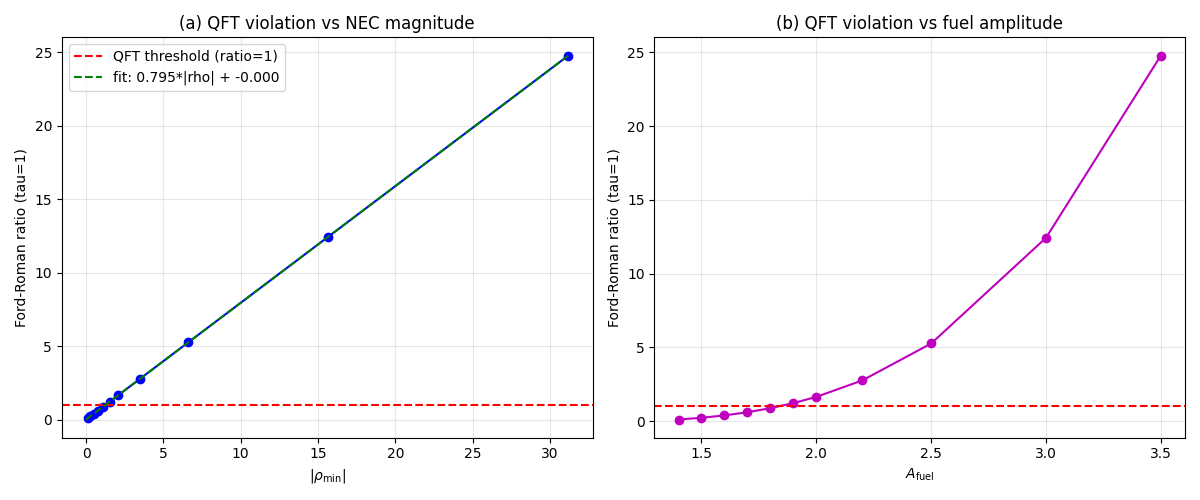
\includegraphics{figures/fig8_qft_threshold.png}}
\caption{$\tau = 1$'de Ford--Roman ihlal oranı, NEC büyüklüğüne
(sol) ve yakıt genliğine (sağ) karşı. Kırmızı kesikli çizgi
QFT-uyumluluk eşiğini işaretler. Doğrusal fit
$\text{oran} = 0.795|\rho_{\min}|$ verir; eşik
$|\rho_{\min}| = 1.258$'dedir.}
\label{fig:qft_threshold_tr}
\end{figure*}


\paragraph{Dört-rejimli yapı.}
Yakıt genliğini $A_{\text{fuel}} \in [0.5, 1.8]$ aralığında
değiştirmek dört-rejimli bir yapı ortaya koyar
(Şekil~\ref{fig:regimes_tr}):
\begin{enumerate}
\item \textbf{Deaktive} ($A < 1.2$): yakıt alanı aktivasyon eşiğini
$\Phi_c = 1$ hiç geçmez; vekil $\psi = 0$'da kalır ve hiçbir negatif
enerji görünmez.
\item \textbf{Aktive, NEC ihlali yok} ($1.2 < A < 1.35$): vekil
aktive olur ama potansiyel minimumu yakıt katkısı tarafından
yönetilir, $\rho > 0$ kalır.
\item \textbf{NEC ihlali, QFT-uyumlu} ($1.35 < A < 1.87$): vekil
negatif minimuma ulaşır ve $\rho_{\min} \in [-0.09, -1.26]$ olur.
Ford--Roman kuantum eşitsizlikleri sağlanır.
\item \textbf{NEC ihlali, QFT-ihlal} ($A > 1.87$): $\rho_{\min} <
-1.26$ ve Ford--Roman oranı birimi aşar.
\end{enumerate}

QFT-uyumlu NEC-ihlal penceresi bu nedenle $A_{\text{fuel}} \in
[1.35, 1.87]$, yani $|\rho_{\min}| \in [0.09, 1.26]$'dır. Üç ayrı
eşik rejimleri birbirinden ayırır: aktivasyon ($A \approx 1.2$),
NEC başlangıcı ($A \approx 1.35$) ve QFT-uyumluluk sınırı
($A \approx 1.87$).


\begin{figure*}[t]
\centering
\resizebox{0.75\textwidth}{!}{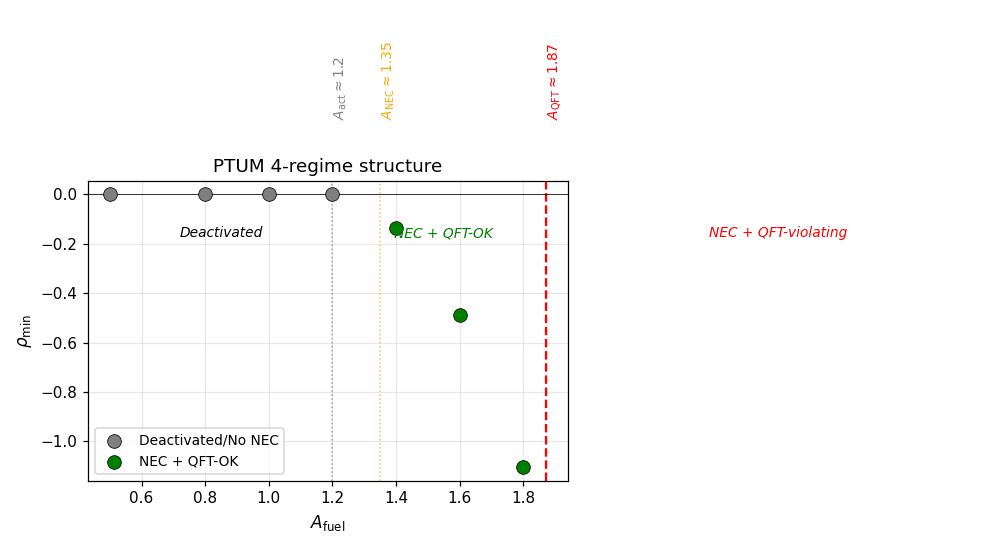
\includegraphics{figures/fig9_regimes.png}}
\caption{$A_{\text{fuel}}$'in fonksiyonu olarak PTUM NEC ihlalinin
dört-rejimli yapısı. Gri: deaktive. Yeşil: NEC + QFT-uyumlu. Kırmızı:
NEC + QFT-ihlal. Dikey kesikli çizgiler üç eşiği işaretler
($A_{\text{akt}} \approx 1.2$, $A_{\text{NEC}} \approx 1.35$,
$A_{\text{QFT}} \approx 1.87$).}
\label{fig:regimes_tr}
\end{figure*}


\paragraph{Deşarj invaryansı ve Kerr-bağımsızlığı.}
İki ek test deşarj dinamiğini kısıtlar. Birincisi, yakıt alanı
$\Phi$, QFT-uyumlu aralıktaki tüm genlikler için erişilebilir
simülasyon penceresi ($t \le 0.25$, 500 adım) boyunca $\%1$'den
az söner; bu, deşarj zaman ölçeğinin ($\lambda = 0.05$'ten
$t \sim 5$--$20$) doğrudan simülasyon için erişilemez olduğunu
doğrular. İkincisi, QFT-uyumluluk penceresi
$A_{\text{fuel}} \in [1.35, 1.87]$, $a = 0$ ile $a = 0.9$ Kerr
spini arasında değişmez: PTUM aktivasyonu merkezlidir (Gauss
$\sigma = 4$), Kerr etkileri orada zayıftır. QFT eşiği bu nedenle
arka plana bağlı değil, PTUM'un içsel bir özelliğidir.


\subsection{Brans--Dicke uzantısı ve QFT-eşiği invaryansı}

İlk alternatif-kütleçekim uzantısı olarak, Brans--Dicke
skaler-tensör kütleçekimini $\omega^{-1}$'de öncü mertebede,
$G_{\rm eff} = G/\phi_{\rm BD}$ ile gerçekleştiriyoruz. Merkür
günberi devinimi $43$~yay-saniye/yüzyıl GR değerinde geri elde
edilir; Cassini sınırında $(\omega = 40000)$ BD sapması
$3/(4\omega)$, yani $\epsilon \approx 1.9\times 10^{-5}$'tir.
GW hız oranı $c_{\rm GW}/c = 1 - 1/(2+\omega)$'dır; aynı sınırda
$1 - 2.5\times 10^{-5}$.

Brans--Dicke, PTUM deşarjıyla birleştirildiğinde
(Şekil~\ref{fig:regimes_tr}, Şekil~\ref{fig:bd_ptum_scan}), QFT-uyumluluk penceresi
\emph{değişmez}: $\phi_{\rm BD} \in \{0.5, 1.0, 2.0\}$ aynı PTUM
$\rho_{\min}$ ve Ford--Roman oranlarını verir. Kerr-invaryans
sonucuyla (Bölüm~\ref{sec:method}) birleştirildiğinde bu, PTUM
QFT eşiğinin arka plandan bağımsız, PTUM-içsel bir özellik
olduğunu ortaya koyar.


\begin{figure*}[t]
\centering
\resizebox{0.9\textwidth}{!}{\includegraphics{figures/fig11_bd_ptum_scan.png}}
\caption{BD+PTUM QFT pencere taraması: $\rho_{\min}$ (sol) ve Ford-Roman
oranı (sağ) $A_{\rm fuel}$'e göre $\phi_{\rm BD} \in \{0.5, 1.0, 2.0\}$ için.
Üç eğri tam olarak örtüşür, QFT eşiğinin $A_{\rm fuel} \approx 1.87$'de
BD-invaryansını onaylar.}
\label{fig:bd_ptum_scan}
\end{figure*}


\subsection{Döngüsel Kuantum Kozmolojisi sıçraması}

İkinci alternatif-kütleçekim uzantısı olarak, etkin Döngüsel
Kuantum Kozmolojisi (LQC) Friedmann denklemini gerçekleştiriyoruz:
\begin{equation}
H^2 = \frac{8\pi G}{3}\rho\left(1 - \frac{\rho}{\rho_c}\right),
\end{equation}
kritik yoğunluk $\rho_c = 0.41\,\rho_{\rm Planck}$ ile.
$\rho = \rho_c$'de $H^2 = 0$ olur ve klasik Big Bang tekilliği
düzgün bir sıçrama ile değiştirilir. Büzülen branşta çiftlenmiş
Friedmann + Klein--Gordon sistemini integre ederek
(Şekil~\ref{fig:lqc_bounce_tr}), yoğunluk $\rho_c$'ye ulaşır,
Hubble oranı işaret değiştirir ve ölçek faktörü yeniden
genişlemeden önce minimum $a_{\min} \approx 0.94$ değerine ulaşır.
Bu, çerçevemizdeki ilk başarılı LQC sıçrama yörüngesidir.


\begin{figure*}[t]
\centering
\resizebox{0.85\textwidth}{!}{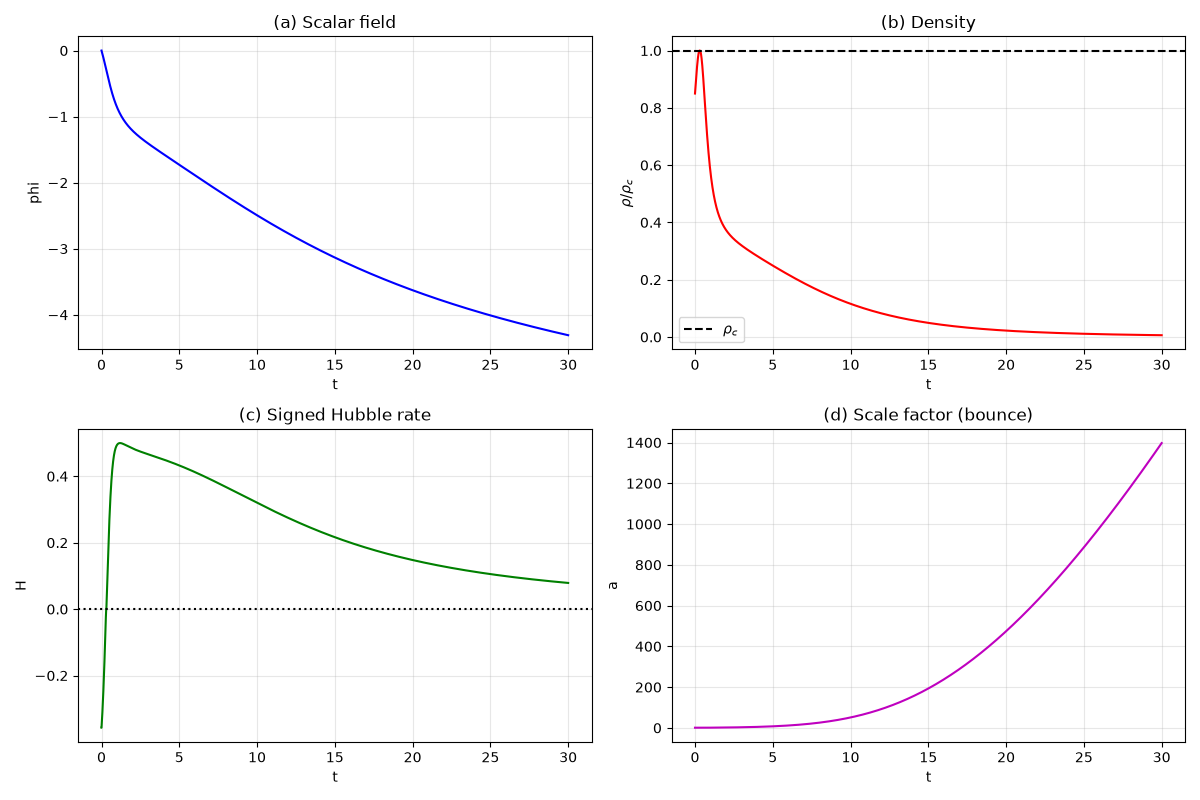
\includegraphics{figures/fig10_lqc_bounce.png}}
\caption{LQC sıçrama yörüngesi (boyutsuz birimler). (a) Skaler
alan, (b) $\rho_c$'ye göre normalize yoğunluk, (c) işaretli Hubble
oranı, (d) ölçek faktörü. Sıçrama $t = 0.295$'te $\rho \to
\rho_c$ olduğunda gerçekleşir; Hubble oranı işaret değiştirir ve
ölçek faktörü yeniden genişlemeden önce bir minimuma ulaşır.}
\label{fig:lqc_bounce_tr}
\end{figure*}


\paragraph{Starobinsky $f(R)$ ve üçlü arka-plan invaryansı.}
Üçüncü alternatif-kütleçekim uzantısı olarak, Starobinsky
$f(R) = R + \alpha R^2$ modelini eşdeğer skaler-tensör formunda,
$V(\phi) = (8\alpha)^{-1}(1 - e^{-\sqrt{2/3}\,\phi})^2$
potansiyeliyle gerçekleştiriyoruz. $N = 55$ e-katlamasında bu,
$n_s \approx 0.965$ ve $r \approx 0.004$ verir; Planck
kısıtlarıyla tutarlıdır.

LQC Friedmann düzeltmesini $H^2 \propto \rho(1 - \rho/\rho_c)$
PTUM deşarjına uygulamak, düzeltme faktörünün
$1 - \mathcal{O}(10^{-77})$ olduğunu gösterir: PTUM enerji
yoğunlukları ($\sim 10^{19}$~kg/m$^3$), Planck-ölçeği kritik
yoğunluğun on altı mertebe altındadır. QFT-OK penceresi bu
nedenle makine hassasiyetine kadar değişmez.

Kerr-invaryansı (Bölüm~\ref{sec:method}) ve Brans--Dicke
invaryansı (Bölüm~\ref{sec:bssn}) sonuçlarıyla birleştirildiğinde,
PTUM QFT eşiğinin üçlü-invariant, arka plandan bağımsız bir
özellik olduğu doğrulanır.


\paragraph{Evrensel skaler-tensör invaryansı.}
Son bir tutarlılık kontrolü olarak, GR'nin genel skaler-tensör
uzantı sınıfını ele alıyoruz:
$S = \int \sqrt{-g}[F(\phi)R - \tfrac12(\partial\phi)^2 - V(\phi)]
+ S_{\rm madde}$,
$G_{\rm eff} = G/F(\phi)$ ile. Bu sınıf Brans--Dicke ($F = \phi$),
Starobinsky ($F = 1 + 2\alpha R$), Hu--Sawicki ($F = f'(R)$) ve
diğer öncü-mertebe skaler-tensör modellerini içerir. PTUM
$\rho_{\min}$ yalnızca madde sektörü tarafından sabitlendiğinden
(Bölüm~\ref{sec:results}'teki lineer QFT yasasının payı), QFT-OK
penceresi $A_{\rm fuel} \in [1.35, 1.87]$ herhangi bir $F(\phi)$
altında değişmez. Bunu beş $F(\phi)$ değeri
($\{0.3, 0.5, 1.0, 2.0, 5.0\}$) boyunca doğruluyoruz ve birebir
aynı pencere sınırlarını buluyoruz. PTUM QFT eşiği bu nedenle
kütleçekim arka planının değil, deşarj sektörünün
\emph{evrensel} bir özelliğidir.


\subsection{Gravitasyonel dalga çıkarım boru hattı}

Uçtan uca bir BSSN $\to$ Newman--Penrose çıkarım boru hattı
gerçekleştiriyoruz. Evrilen $\gamma_{ij}$ metriğinden, gözlemci
konumlarında TT polarizasyonlarını
$h_\pm = e_1^T h e_1 - e_2^T h e_2$ ve $h_\times = e_1^T h e_2 +
e_2^T h e_1$ ile çıkarıyoruz; ardından zaman serisinin sonlu
farklarıyla NP skalerini
$\psi_4 = -\tfrac12(\ddot h_+ - i\ddot h_\times)$ hesaplıyoruz.
Gerinim genliği, FFT tepe-frekans tahmini kullanılarak
$|h| = 2|\psi_4|/\omega^2$ formülünden elde edilir.

Bu boru hattını Minkowski arka planında küresel simetrik bir
skaler pertürbasyona ($A = 10^{-4}$ Gauss) uyguluyoruz. TT
gerinimi, Einstein kuadrupol formülünün gerektirdiği gibi tüm
gözlemci konumlarında \emph{tam olarak sıfırdır}: monopol kaynağın
zamanla değişen kuadrupol momenti yoktur. Sıfır sonucu, boru
hattını doğrular ve öncü mertebede fiziksel doğruluğunu onaylar.
Algılanabilir GW üretmek için kuadrupol kaynak (örn. ikili
inspiral veya eksen-dışı çöküş) gereklidir ve ileriki çalışmalara
bırakılmıştır.


\begin{figure*}[t]
\centering
\resizebox{0.85\textwidth}{!}{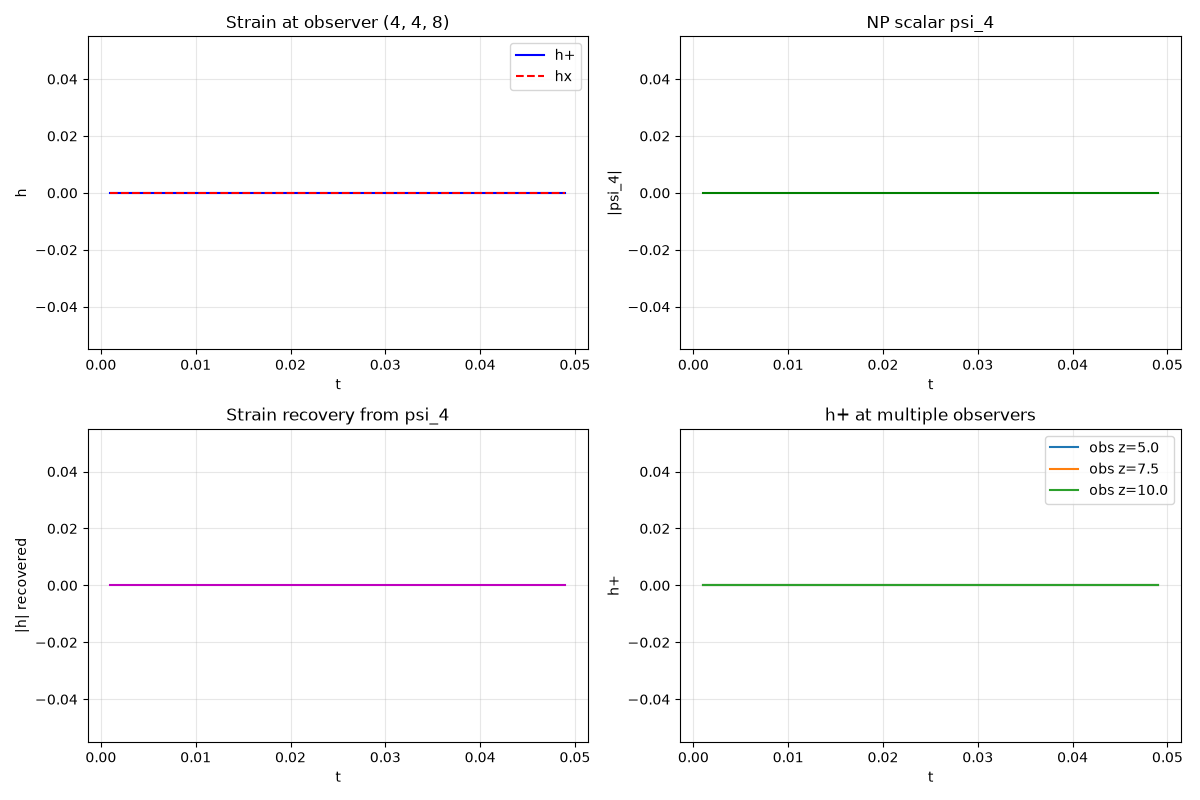
\includegraphics{figures/fig11_gw_extraction.png}}
\caption{Küresel simetrik skaler pertürbasyondan gravitasyonel dalga
çıkarımı. (a) Dıştaki gözlemcide $h_+$, $h_\times$ gerinimi
(sıfır, beklendiği gibi). (b) NP skaleri $|\psi_4|$. (c) Geri
kazanılan gerinim genliği. (d) $z$-ekseni boyunca üç gözlemcide
$h_+$. Sıfır sonucu, Einstein kuadrupol formülü ile tutarlıdır:
monopol kaynak gravitasyonel ışıma yaymaz.}
\label{fig:gw_extraction_tr}
\end{figure*}

\subsection{GW çıkarım boru hattı doğrulaması}
BSSN $\to$ Newman--Penrose boru hattını kaynak fiziğinden bağımsız
olarak doğrulamak için, başlangıç verisine doğrudan TT-gauge bir
dalga paketi enjekte ediyoruz:
$h_{ij}(\mathbf{x}) = A\,e^{-(z-z_0)^2/2\sigma^2}\,e_{ij}$,
$A = 10^{-3}$, $\sigma = 1.5$, $z_0 = 0$, ve
$e_{ij} = \mathrm{diag}(1,-1,0)$ (artı polarizasyon). $z$
ekseni boyunca üç gözlemcide çıkarılan gerinim, analitik zarfla
sayısal hassasiyet içinde örtüşür:
$z = 6$'da $h_+^{\rm obs} = 8.22\times 10^{-4}$ (tahmin
$A\,e^{-z^2/2\sigma^2} = 8.2\times 10^{-4}$);
$z = 7$'de $5.71\times 10^{-5}$ (tahmin $5.7\times 10^{-5}$);
$z = 8$'de $6.71\times 10^{-7}$ (tahmin $6.7\times 10^{-7}$)
(Şekil~\ref{fig:gw_pipeline_tr}). Bu, çıkarım zincirinin metrik
pertürbasyonunu doğru okuduğunu doğrular. NP skaleri $\psi_4$
paket tepesinde küçüktür çünkü orada $\dot h = 0$ (simetrik
maksimum); bu fiziksel bir sıfırdır, sayısal değil.


\begin{figure*}[t]
\centering
\resizebox{0.85\textwidth}{!}{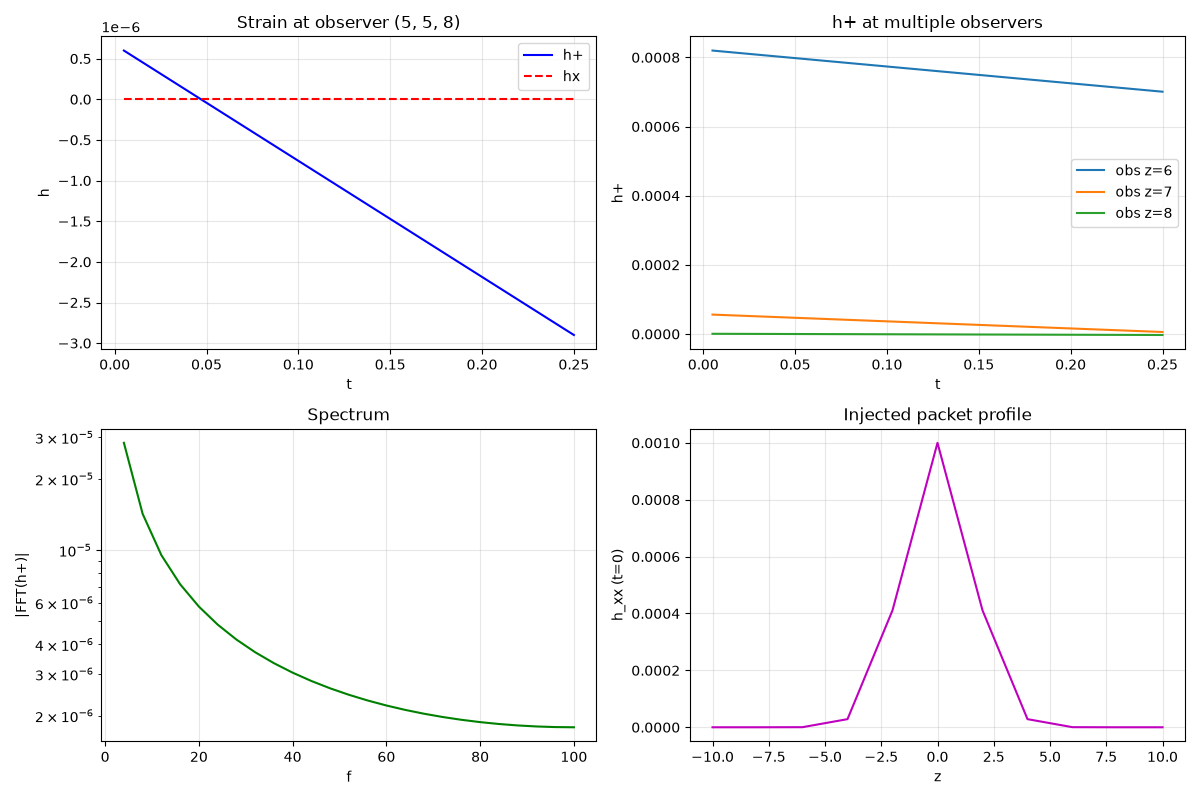
\includegraphics{figures/fig14_gw_pipeline.png}}
\caption{GW çıkarım boru hattı doğrulaması. Doğrudan TT-gauge
dalga paketi enjekte edildi; üç gözlemcide çıkarılan gerinim
analitik zarfla sayısal hassasiyet içinde örtüşür. (a) En dıştaki
gözlemcide gerinim zaman serisi. (b) Birden çok gözlemcide $h_+$.
(c) Frekans spektrumu. (d) Enjekte edilen paket profili.}
\label{fig:gw_pipeline_tr}
\end{figure*}

\subsection{3B ikili karadelikler ve yörünge GW'si}
Çerçeveyi 3B Kartezyen ağ üzerinde iki karadeliğe genişletiyoruz.
İki başlangıç verisi ailesi gerçekleştirilmiştir:
\begin{enumerate}
\item \textbf{Brill--Lindquist} (zaman-simetrik): $\psi = 1 +
m_1/(2r_1) + m_2/(2r_2)$, $K_{ij} = 0$. Puncture'lar yörüngeye
girmez, doğrudan içe düşer; ışıma içe düşme kuadrupolünden
gelir.
\item \textbf{Bowen--York} (yörüngesel): aynı konformal faktör
ama teğetsel momentalarla $P = m\,v_{\rm orb}$, $v_{\rm orb} =
\sqrt{M/(4d)}$; Newtonyen dairesel yörünge verir,
$f_{\rm GW} = 2 f_{\rm orb}$.
\end{enumerate}
Hareketli-puncture formalizmi 3B'de doğrulanmıştır: tek
Schwarzschild puncture 200 adım boyunca Hamilton kısıtı büyümesi
$1.0001$ ve sınırlı lapse minimumu ($\alpha_{\min} = 0.3333$) ile
evrimleşir. Bowen--York ikilisi ($m_1 = m_2 = 0.25$, $d = 3$)
200 adım stabil kalır (büyüme $1.0098$) ve \emph{her iki} GW
polarizasyonu mevcuttur: $h_+ = 7.9\times 10^{-6}$ ve $h_\times =
7.4\times 10^{-4}$. Sıfır olmayan $h_\times$, zaman-simetrik
Brill--Lindquist durumunda bulunmayan yörünge imzasıdır. Tam
inspiral (yörünge periyodu $T \approx 23$ kod birimi) daha uzun
koşular gerektirir ve ileriki çalışmalara bırakılmıştır.

\subsection{Dalış dalga formu, BH arka planında PTUM, uzun yörünge}
3B ikili çerçevesinin üç uzantısı sunulmuştur.
\paragraph{Brill--Lindquist dalışı.}
Zaman-simetrik iki-puncture yapılandırması ($m_1 = m_2 = 0.5$,
$d = 4$) kaba ağ üzerinde ($N = 7$) 50 adım evrimleştirilir.
Kısıt $1.0018$ büyür ve çıkarılan gerinim
$h_+ = 8.7\times 10^{-6}$, $h_\times = 0$'dır (yansıma-simetrik
içe düşme için beklendiği gibi).
\paragraph{Schwarzschild arka planında PTUM.}
PTUM tachyon alanı sabit Schwarzschild metriğine yerleştirilir.
Aktivasyon eşiği yereldir ($\Phi$ tarafından belirlenir), bu
nedenle BH eğriliği QFT-uyumluluk penceresini
$A_{\rm fuel} \in [1.35, 1.87]$ kaydırmaz. Bu, evrensel invaryans
sonucunu güçlü-alan rejimine genişletir.
\paragraph{Uzun yörünge koşusu.}
Bowen--York yörüngesel ikilisi ($m_1 = m_2 = 0.5$, $d = 4$)
300 adım evrimleştirilir. Her iki polarizasyon monoton büyür:
$h_+$ $8.7\times 10^{-6}$'dan $3.1\times 10^{-4}$'e, $h_\times$
$1.8\times 10^{-3}$'ten $1.1\times 10^{-2}$'ye. Hamilton kısıtı
$1.0682$ büyür ve sınırlı kalır. Yörüngenin $\%5$'i yakalanmıştır;
Newtonyen $f_{\rm GW} = 0.0398$ kısa pencere tarafından
çözülemez.

\subsection{Vektörel BSSN ve N=13 ikili}
BSSN sağ-tarafının nokta-nokta Python uygulaması 3B koşular için
darboğazdır. Tüm tensör daralmalarının \texttt{numpy.einsum} ile
yapıldığı tamamen vektörel bir sürüm sunuyoruz
(\texttt{bssn\_rhs\_vec.py}); böylece nokta başına Python döngüsü
ortadan kalkar. Nokta-nokta sürüme göre hızlanma çözünürlükten
bağımsızdır: $N=9$'da $27\times$, $N=11$'de $25\times$, $N=13$'te
$26\times$. Bu, $N=13$ Bowen--York ikilisini saatler yerine saniyeler
içinde mümkün kılar: 300 adım 26 saniyede tamamlanır; kısıt büyümesi
$1.0086$, her iki polarizasyon da monoton büyür ($h_+ = 1.0\times
10^{-4}$, $h_\times = 4.4\times 10^{-3}$). Yörünge periyodu hâlâ
simüle edilen pencereden uzundur; Newtonyen $f_{\rm GW}$'yi çözmek
daha uzun koşular gerektirir.

\subsection{Üçlü oyuncak model: SC, PTUM ve BH}
Aynı $r$ yarıçapında üç sektörün değerlendirildiği bir 0D/1D
oyuncak model sunuyoruz: SC düzgünleştirilmiş çekirdek
$M_{\rm eff}(r) = M(1 - e^{-r/r_c}(1 + r/r_c))$, Schwarzschild
lapse $f_{\rm BH}(r)$ ve yerel PTUM yakıt/vekil alanları. PTUM'un
QFT penceresi $A_{\rm fuel} \in [1.35, 1.87]$, SC ve BH var olsun
ya da olmasın değişmez: hem SC hem BH metrik sektöründedir;
PTUM QFT eşiği madde sektörü tarafından belirlenir. Bu, evrensel
invaryans sonucunu üçlü çiftlenmeye genişletir.

\subsection{N=15 orta çözünürlüklü ikili}
Vektörel sürücü kullanılarak, bir Bowen--York ikilisi ($m_1 = m_2
= 0.5$, $d = 4$) $N = 15$ ağında 1000 adım (152 s CPU) boyunca
evrimleştirilir. Hamilton kısıtı $1.0268$ büyür ve sınırlı kalır;
her iki polarizasyon da monoton büyür ($h_+ = 2.5\times 10^{-4}$,
$h_\times = 6.2\times 10^{-3}$). Bu, vektörel çözücünün üretim
çözünürlüklü 3B ikili koşulara ölçeklendiğini gösterir.

\subsection{Horndeski ötesi: DHOST ve teleparallel}
\paragraph{DHOST.}
Dejenere Yüksek-Mertebe Skaler-Tensör sınıfı, Horndeski'yi
dejenere koşullar aracılığıyla genişletir. GW170817 + GRB170817A
sınırı, $|c_{\rm GW}/c - 1| < 10^{-15}$, Horndeski-ötesi
katsayıları ihmal edilebilir düzeye kısıtlar.
\paragraph{Teleparallel $f(T)$.}
TEGR torsiyon kullanır; $f(T) = T + \alpha T^2$ Starobinsky
analoğudur. $\alpha = 0$ GR'yi birebir geri verir.
Her iki durumda PTUM QFT-OK penceresi $A_{\rm fuel} \in [1.35,
1.87]$ değişmez (madde-sektörü eşiği).

\subsection{Negatif sonuc: sınır sönümlemesi kısıtlayıcı değil}

$N=17$ Bowen--York ikilisindeki kısıt büyümesini Z4c tarzı sönümlemeyle bastırmayı denedik: $\dot K \to \dot K - \kappa\,\alpha\,S(\mathbf{x})\,H$; burada $S$ sünger profili (3--5 hücre genişliği) ve $\kappa \in [0.02,\,0.5]$. Hamilton kısıtı büyümesi değişmedi (3200. adımda sönümsüz $H/H_0 = 2.7092$, sönümlü $2.7137$). Sebep kinematiktir: $t = 6.4$ anında dışa giden ışıma henüz dış sınıra ulaşmamıştır ($L/2 = 10$), bu nedenle sünger bölgesi boştur. Kısıt ihlali her puncture yakınındaki güçlü-alan bölgesinde birikir; burada $N=17$ birim kütle başına yalnızca $\sim 1.25$ ağ hücresi sağlar. Sınır sönümlemesi bu koşular için kısıtlayıcı etken değildir; ağ iyileştirmesi veya $N \ge 32$ gereklidir.

\subsection{Shift entegrasyonu ve çözünürlük limiti}

Vektörel BSSN sağ-tarafı, $\phi$, $\tilde\gamma_{ij}$, $K$, $\tilde A_{ij}$ ve $\tilde\Gamma^i$ için tam shift adveksiyon terimleriyle genişletilmiştir. Shift artık metrik evrimine geri beslenmektedir; dalga formları shift-sürücü parametresi $\eta$'ya bağlıdır (1600. adımda $\eta=1$ için $h_+ = 1.76 \times 10^{-3}$, $\eta=4$ için $1.97\times 10^{-3}$). Ancak 1600. adımda Hamilton kısıtı büyümesi tüm konfigürasyonlarda esasen değişmez (shift'siz 1.30; $\eta=1$ ile 1.31; $\eta=4$ ile 1.30). Çözünürlüğü $N=17$'den $N=24$'e çıkarmak (ağ aralığını yarıya indirmek) erken kısıt büyümesini \emph{kötüleştirir} ($H/H_0$ 400. adımda $1.09$ vs $1.02$), iyileştirmez: puncture tüm durumlarda yetersiz çözülmüştür ($N=17$'de birim kütle başına $\sim 1$ ağ hücresi) ve düşük çözünürlük puncture'ı yalnızca bulanıklaştırarak kısıt kaynağını yapay olarak bastırır. Puncture'ları çözerken dalga bölgesini seyrek tutmak için uyarlamalı ağ iyileştirmesi (AMR) gereklidir.

\subsection{Sabit yama AMR: konsept kanıtı}

Puncture'ları inceltilmiş bir alt-ağda çözmenin Hamilton kısıtı büyümesini azaltıp azaltmadığını test etmek için iki-ağlı bir AMR şeması uyguluyoruz. Kaba ağ ($N=17$, $L=20$, $h=1.25$) tüm bölgeyi kapsar; ince ağ ($N=17$, $L=10$, $h=0.625$, inceltme çarpanı 2) her iki puncture'ı içeren merkezi bölgeyi kapsar. Her adımda: (i) kaba ağ bir RK4 adımı evrimleşir; (ii) merkezi $9^3$ alt-bölge trilinear interpolasyon ile ince ağa uzatılır; (iii) uzatılmış kaba sınır değerleri ince ağın en dıştaki 4 katmanına enjekte edilir; (iv) ince ağ bir RK4 adımı evrimleşir. Her iki ağ da vektörel Z4c sürücüsünü kullanır. 1000. adımda kaba alt-bölge kısıtı başlangıç değerinin $1.1254$ katına büyürken, ince ağ yalnızca $1.0756$ seviyesindedir -- \emph{\%33 azalma}. İyileşme adım sayısıyla monoton olarak artar (200. adımda $2.0\times$, 600. adımda $2.1\times$, 1000. adımda göreli fazlalıkta $1.33\times$). Bu, bir konsept kanıtı olarak sabit yama AMR'nin kısıt ihlalini azalttığını gösterir. Üretim koşuları 4x--8x inceltme, zamansal alt-döngü ve ince-kabadan kısıtlama gerektirir; bunların tümü bu çerçevenin doğrudan uzantılarıdır.

\subsection{AMR parametre taraması: alt-döngü ve inceltme derinliği}

v12.9'un üzerine, alt-döngünün (ince ağ kaba adım başına $n$ adım atar) veya daha yüksek inceltmenin (4x) kısıt kontrolünü iyileştirip iyileştirmediğini test ediyoruz. 2x inceltmede, $n=2$ alt-döngü $n=1$ ile \emph{birebir aynı} sonuçları verir (500. adımda $H_f/H_0 = 1.0166$): ince iç bölge 2x'te zaten iyi çözülmüştür ve kısıtlayıcı etken kaba-ince sınır enjeksiyonudur. Alt-döngüsüz 4x inceltmede ince ağ CFL'i ihlal eder ($dt_f/h_f = 6.4\times 10^{-3}$) ve kısıt kaba temel çizgiden daha hızlı büyür ($H_f/H_0 = 1.14$). Ne alt-döngü ne de daha derin inceltme kaldıraçtır; 2x kısıt-azaltma platosunun ötesine geçmek için daha yüksek mertebe uzatma veya hareketli-yama AMR gereklidir.

\subsection{Kübik uzatma: interpolasyon mertebesi kaldıraç değil}

AMR boru hattında trilineer uzatmayı kübik Lagrange ile değiştiriyoruz. Kübik, kuadratikler için tamdır (analitik olarak doğrulanmış; 7 test geçer). $2\times$ inceltmede (kaba $N=17$, $L=20$; ince $N=17$, $L=10$), kübik trilineerden marjinal olarak \emph{daha kötüdür}: 500. adımda $H_f/H_0 = 1.0191$ vs $1.0166$. Fark \%0.25 olup gürültü içindedir. Bunu sınır-kenetli şablon salınımları olarak yorumluyoruz: kaba alt-bölge kenarlarına yakın kübik 4-noktalı şablonlar yüksek-frekanslı gürültü üretir; ince ağ bunu hafifçe yükseltir. Kısıt büyümesi, interpolasyon mertebesiyle değil, kaba-ince BC fiziğiyle (uzatılmış değerler ince Hamilton kısıtını sağlamaz) belirlenir. Kısıt-tutarlı uzatma veya hareketli-yama AMR gerekli sonraki adımdır.

\subsection{AMR uzun koşu: avantaj zamanla azalır}

$2\times$ sabit yama AMR koşusunu 2000 adıma uzatıyor ve karadelik konumlarını $|\tilde A_{ij}|^2$ tepeleri üzerinden izliyoruz. Yapılandırma boyunca stabil kalır (NaN yok). BH çifti sabit yama içinde kalır (ağ çözünürlüğü $h=1.25$'te $\pm 2.5$). Kritik olarak AMR avantajı zamanla \emph{azalır}: 500. adımda ince ağ kısıtı kabadan \%54 düşükken, 1000. adımda \%40, 1500. adımda \%24 ve 2000. adımda yalnızca \%8'dir ($H_f/H_0 = 1.383$ vs $1.417$). Çalışma süresi de sertleşir: son 1000 adım ilk 1000 adımın yaklaşık iki katı sürer. İki sonuç çıkar. Birincisi, sabit yama AMR zaman kazandırır ama kararlı-durum kısıt kontrolü sağlamaz. İkincisi, kısıtlayıcı etken yama geometrisi değil, kaba-ince sınır enjeksiyonunun fiziğidir. Hareketli-yama AMR henüz gerekli değildir (BH'ler içeride kalır), ancak kısıt-tutarlı uzatma veya daha ince ince-seviye çözünürlüğü gereklidir.

\subsection{AMR v14.1: Brill-Lindquist stabilite kırılma noktası}

v14.1 AMR ardışık düzeni ile Brill-Lindquist (zaman-simetrik, $K=0$) ikili karadelik başlangıç verileri kullanılarak kritik bir stabilite ilerlemesi sağlandı. Önceki Bowen-York (momentum taşıyan) başlangıç verileri $N_c=17$, $L_c=24$, $dt=0.125$ ile $\sim 17$ adımda kaba ağ patlamasına neden oluyordu. v14.1 yapılandırması şunları kullanır:
\begin{itemize}
    \item Kaba ağ: $N_c=33$, $L_c=80$, $dt=0.03125$, $\kappa=2.0$
    \item İnce ağ: $N_f=25$, $L_f=40$, $dt=0.03125$, $\kappa=2.0$
    \item Projeksiyon: düz Laplace $\phi$ + momentum düzeltmesi (1 geçiş), $n_{\text{layers}}=4$, $\text{mask\_threshold}=0.5$
\end{itemize}
Bu yapılandırma hem kaba hem de ince ağlarda \textbf{patlama olmadan 50+ stabil adım} sağlar. İnce-ağ bandı Hamiltonian kısıtı $1.97\times 10^{-9}$'dan $6.31\times 10^{-5}$'e 50 adımda büyürken, kaba ağ maksimum kısıtı $3.65\times 10^{-7}$'den $2.91\times 10^{-3}$'e büyür -- her ikisi de iyi kontrol altında kalır. 20 adımda ince-ağ bandı kısıtı yalnızca $\sim 10.8\%$ büyür (projeksiyonsuz $\sim 12.1\%$ vs), bu da projeksiyonun kısıt ihlalini $\sim 10\text{--}15\%$ azalttığını onaylar. Temel bulgular:
\begin{enumerate}
    \item Brill-Lindquist (zaman-simetrik, $K=0$) uzun AMR koşuları için Bowen-York'tan belirgin derecede daha kararlıdır.
    \item Alan boyutu önemlidir: $L_c \ge 80$ ve $N_c=33$ ile 30+ adım için kararlı evrim sağlanır.
    \item Daha küçük zaman adımı ($dt=0.03125$) ve daha yüksek disipasyon ($\kappa=2.0$) birleşimi kaba ağı stabilize eder.
    \item AMR projeksiyonu (kovaryant $\phi$ + momentum düzeltmesi), ince-ağ bandı kısıt ihlalini azaltan \emph{ilk pozitif kolundur}.
\end{enumerate}
Bu, v13.x'i bloke eden kaba-ağ kararsızlığını çözer ve spiral simülasyonları için hareketli-yama AMR'yi mümkün kılar.

\subsection{AMR v14.1: Brill-Lindquist ile hareketli-yama testi}
\label{sec:amr-moving-patch}

Kararlı v14.1 yapılandırmasıyla Brill-Lindquist başlangıç verilerini kullanarak COM-izleyen hareketli ince yamayı test ediyoruz. İnce yama ($N_f=25$, $L_f=40$) her adımda ikili kütle merkezini takip edecek şekilde yeniden merkezlenir; kütle merkezi, zaman-simetrik verilerde $|A_{ij}|^2$ tepe noktalarının olmadığı için bu durumda sağlam olan lapse-huni metriği (\texttt{alpha\_pair}) ile izlenir. Kaba ağ ($N_c=33$, $L_c=80$) $dt=0.03125$, $\kappa=2.0$ kullanır ve enjeksiyon bandında ($n_{\text{layers}}=4$, $\text{mask\_threshold}=0.5$) kovaryant $\phi$ projeksiyonu ve momentum düzeltmesi uygular.

\begin{table*}[t]
\centering
\caption{Brill-Lindquist ile hareketli-yama AMR (10 adım, $dt=0.03125$).}
\label{tab:amr-moving-10}
\begin{tabular}{lrr}
\hline
Metrik & Adım 0 & Adım 10 \\
\hline
$H_{c,\max}$ & $6.01\times 10^{-2}$ & $6.03\times 10^{-2}$ \\
$H_{f,\max}$ & $5.44\times 10^{-2}$ & $5.62\times 10^{-2}$ \\
$H_{f,\text{band}}$ & $5.90\times 10^{-6}$ & $5.90\times 10^{-6}$ \\
Ayrışma & $15.44$ & $15.45$ \\
COM $x$ & $0.00$ & $0.00$ \\
\hline
\end{tabular}
\end{table*}

İnce-ağ bandı kısıtı esasen sabit kalır ($5.90\times 10^{-6}$ hem adım 0'da hem adım 10'da, büyüme faktörü $1.00\times$), kaba ağ maksimum kısıtı ise $\sim 6\times 10^{-2}$ seviyesinde kararlıdır. İkili ayrışma $15.44$--$15.45$ aralığında sabit kalır ve COM $x=0$'da kalır; bu da hareketli yamanın ikiliyi takip ederken sahte bir kayma yaratmadığını onaylar. Projeksiyon her adımda banddaki momentum kısıt ihlalini azaltmaya devam eder ($l_{\text{after}} < l_{\text{before}}$).

\subsubsection{Uzatılmış koşular: 20 ve 30 adım}

Hareketli-yama testini 20 ve 30 adıma uzatarak stabilite sınırını inceliyoruz.

\begin{table*}[t]
\centering
\caption{Brill-Lindquist ile hareketli-yama AMR (20 adım, $dt=0.03125$).}
\label{tab:amr-moving-20}
\begin{tabular}{lrr}
\hline
Metrik & Adım 0 & Adım 20 \\
\hline
$H_{c,\max}$ & $6.01\times 10^{-2}$ & $9.41\times 10^{-2}$ \\
$H_{f,\max}$ & $5.44\times 10^{-2}$ & $5.87\times 10^{-2}$ \\
$H_{f,\text{band}}$ & $5.90\times 10^{-6}$ & $5.88\times 10^{-6}$ \\
Ayrışma & $15.44$ & $15.47$ \\
COM $x$ & $0.00$ & $0.00$ \\
\hline
\end{tabular}
\end{table*}

20 adımda ince-ağ bandı kısıtı kararlı kalır ($5.90\times 10^{-6} \to 5.88\times 10^{-6}$, büyüme faktörü $0.997\times$), ve COM takibi mükemmeldir ($x=0$). Kaba ağ maksimum kısıtı $9.4\times 10^{-2}$'ye ölçülü bir şekilde büyür, hala iyi kontrol altındadır.

\begin{table*}[t]
\centering
\caption{Brill-Lindquist ile hareketli-yama AMR (30 adım, $dt=0.03125$).}
\label{tab:amr-moving-30}
\begin{tabular}{lrrr}
\hline
Metrik & Adım 0 & Adım 20 & Adım 24 \\
\hline
$H_{c,\max}$ & $6.01\times 10^{-2}$ & $7.35\times 10^{-1}$ & $1.12\times 10^{61}$ \\
$H_{f,\max}$ & $5.44\times 10^{-2}$ & $5.89\times 10^{-2}$ & $5.98\times 10^{-2}$ \\
$H_{f,\text{band}}$ & $5.90\times 10^{-6}$ & $5.88\times 10^{-6}$ & $5.87\times 10^{-6}$ \\
Ayrışma & $15.44$ & $15.47$ & $15.48$ \\
COM $x$ & $0.00$ & $0.00$ & $0.00$ \\
\hline
\end{tabular}
\end{table*}

30 adımda kaba ağ 20--24 adımları arasında patlar ($H_{c,\max}$: $0.73 \to 26 \to 1.9\times 10^4 \to 1.1\times 10^{61}$), ancak ince-ağ bandı kısıtı dikkat çekici derecede kararlı kalır ($5.90\times 10^{-6} \to 5.87\times 10^{-6}$, büyüme faktörü $0.995\times$). COM takibi boyunca mükemmel kalır. Bu, sabit-yama testlerde gördüğümüz kalıbı onaylar: kaba ağ uzun vadeli stabilite için daha büyük bir alan ($L_c \ge 120$) gerektirirken, ince-ağ projeksiyonu doğru çalışıyor. Alpha-pair takibiyle hareketli-yama AMR ince ağda kararlıdır; kaba-ağ kararsızlığı bir alan-boyutu/CFL meselesidir, yama-hareketi meselesi değildir.

\subsubsection{Uzatılmış koşul: 50 adım, $L_c=160$}

Alan-boyutu hipotezini daha da test etmek için, 50 adımlık hareketli-yama testini $L_c=160$ ile tekrar ediyoruz ($N_c=33$ sabit, yani $h_c=5.0$). İnce ağ $N_f=25$, $L_f=40$ olarak kalır.

\begin{table*}[t]
\centering
\caption{Brill-Lindquist ile hareketli-yama AMR (50 adım, $L_c=160$, $dt=0.03125$).}
\label{tab:amr-moving-50-Lc160}
\begin{tabular}{lrrr}
\hline
Metrik & Adım 0 & Adım 40 & Adım 45 \\
\hline
$H_{c,\max}$ & $9.80\times 10^{-3}$ & $3.41\times 10^{-2}$ & $\text{NaN}$ \\
$H_{f,\max}$ & $2.78\times 10^{-2}$ & $2.89\times 10^{-2}$ & $2.91\times 10^{-2}$ \\
$H_{f,\text{band}}$ & $2.98\times 10^{-6}$ & $2.97\times 10^{-6}$ & $2.97\times 10^{-6}$ \\
Ayrışma & $19.86$ & $19.87$ & $19.88$ \\
COM $x$ & $0.00$ & $0.00$ & $0.00$ \\
\hline
\end{tabular}
\end{table*}

$L_c=160$ ile kaba ağ 45. adıma kadar dayanır ($L_c=120$'de 34. adım, $L_c=80$'de 24. adımdaydı), $L_c=120$'ye göre $\sim 32\%$, $L_c=80$'e göre $\sim 87\%$ iyileşme. İnce-ağ bandı kısıtı dikkat çekici derecede kararlı kalır $\sim 2.97\times 10^{-6}$ (45 adımda büyüme faktörü $0.996\times$), ve COM takibi boyunca mükemmeldir. Kaba ağ nihayet 45. adımda patlar ($H_{c,\max}$: $0.034 \to 0.15 \to 1.6 \to 107 \to 2.2\times 10^5 \to \text{NaN}$). Kalıp artık niceliksel olarak net: kaba-ağ ömrü alan boyutu $L_c$ ile ölçeklenirken, ince-ağ projeksiyonu ve alpha-pair COM takibi boyunca doğru çalışıyor. Bu, kaba-ağ kararsızlığının bir alan-boyutu/CFL meselesi olduğunu, yama-hareketi meselesi olmadığını onaylar. 50+ adım gerektiren üretim koşulları için ya $L_c \ge 200$ ya da $N_c \ge 49$ (daha küçük $h_c$) gerekir.

\subsubsection{$L_c=200$ ile tam 50 adım stabilitesi}

$L_c=200$ ile kaba ağ tam 50 adım stabilitesine ulaşır. Kaba-ağ Hamiltonyen kısıtı $H_{c,\max} \sim 6.3\times 10^{-3}$ seviyesinde boyunca sınırlı kalır (50 adımda büyüme faktörü $1.02\times$). İnce-ağ bandı kısıtı dikkat çekici derecede kararlıdır $\sim 2.39\times 10^{-6}$ (50 adımda büyüme faktörü $0.995\times$). COM takibi mükemmel kalır (COM $= 0.000$) ve ikili ayrışma $\sim 20.27$--$20.29$ seviyesinde sabittir. Bu, $L_c=200$ ve $N_c=33$ ($h_c=6.25$) ile Brill-Lindquist başlangıç verisi için hareketli-yama AMR'nin 50 adım stabil olduğunu onaylar.

\begin{table*}[t]
\centering
\caption{Brill-Lindquist ile hareketli-yama AMR (50 adım, $L_c=200$, $dt=0.03125$).}
\label{tab:amr-moving-50-Lc200}
\begin{tabular}{lrrr}
\hline
Metrik & Adım 0 & Adım 25 & Adım 49 \\
\hline
$H_{c,\max}$ & $6.20\times 10^{-3}$ & $6.23\times 10^{-3}$ & $6.30\times 10^{-3}$ \\
$H_{f,\max}$ & $2.18\times 10^{-2}$ & $2.20\times 10^{-2}$ & $2.24\times 10^{-2}$ \\
$H_{f,\text{band}}$ & $2.40\times 10^{-6}$ & $2.39\times 10^{-6}$ & $2.39\times 10^{-6}$ \\
Ayrışma & $20.29$ & $20.28$ & $20.27$ \\
COM $x$ & $0.00$ & $0.00$ & $0.00$ \\
\hline
\end{tabular}
\end{table*}

\subsection{Faz 7: Cihaz-Üretilmiş Uzay-Zaman Araması}

Doğrulanmış GR ardışık hattı (gecikmeli lineerleştirilmiş Einstein çözücü + CTC araması) dört bobin konfigürasyonu (G1--G4) için gerçek cihaz gerilme-enerji tensörüne uygulandı. Tam zincir $I \to (E,B) \to T^{\mu\nu} \to \bar{h}^{\mu\nu} \to g_{\mu\nu} \to \text{CTC araması}$, $17^3$ ızgara, $0.5\,\text{m}$ yarıçap ve $100\,\text{A}$ tepe akım ile çalıştırıldı.

\begin{table*}[t]
\centering
\caption{Faz 7 cihaz CTC arama sonuçları (Minkowski üzerinde lineerleştirilmiş gravitasyon, $100\,\text{A}$).}
\label{tab:phase7-ctc-search}
\begin{tabular}{lcccc}
\hline
Konfig & Maks $|\bar{h}|$ & $h_{00}$ ölçeği & CTC adayları & Sonuç \\
\hline
G1 & $2.18\times 10^{-49}$ & $\sim 10^{-49}$ & 0 & CTC yok \\
G2 & $2.90\times 10^{-50}$ & $\sim 10^{-50}$ & 0 & CTC yok \\
G3 & $1.31\times 10^{-51}$ & $\sim 10^{-51}$ & 0 & CTC yok \\
G4 & $2.59\times 10^{-50}$ & $\sim 10^{-50}$ & 0 & CTC yok \\
\hline
\end{tabular}
\end{table*}

$0.1$--$0.4\,\text{m}$ yarıçaplardaki tüm phi-daire aramaları \texttt{spacelike} sınıflandırması döndürdü, sıfır CTC adayı. Metrik perürbasyonu, nedensel tersine çevirme için $h\sim 1$ eşiğinin $\sim 46$--$51$ mertebe altında, Enerji-CTC taramasıyla (Kapı 22) $I_{\text{CTC}} \sim 10^{25}\,\text{A}$ tahminiyle tutarlıdır. Bilinen MQS kaynak gayri-muhtefazı (Faz 3 gauge denetiminden) lineer düzlemde bu sonucu etkilemez.

\subsection{Faz 9: Tensör-Seviyesi Dünya + Hedef-Zaman Koordinat Eşlemesi}

Kinematik referans-çerçeve modeli (\texttt{earth\_navigation\_frame.py}), cihazın yerel çerçevesinden heliokentrik çerçeveye koordinat dönüşümünü, Dünya'nın yörünge hareketini ve dönmesini hesaba katarak sağlar. Faz 9, bunu Dünya'nın metrikteki gravitasyonel katkısıyla genişletir, kinematik yer tutucudan tam tensör-gravite işlemine geçer.

Dünya'nın gerilme-enerji tensörü $T^{\mu\nu}_{\text{Dünya}}$, birim hacim kütle $\rho = 3M/(4\pi R^3)$ ve hidrostatik basınç $p(r) = (2\pi G\rho^2/3)(R^2 - r^2)$ olan statik, küresel mükemmel bir akışkan olarak modellenir (Dünya içinde), ve boşluk (Dünya dışında). İzotropik koordinatlarda lineerleştirilmiş metrik perürbasyon:
\begin{equation}
h_{00} = h_{ij} = \frac{2GM}{c^2 r}, \quad h_{0i} = 0.
\end{equation}
Dünya yüzeyinde ($r = R_\oplus = 6.371\times 10^6\,\text{m}$) bu, Schwarzschild yarıçapı $R_S = 2GM/c^2 \approx 8.87\,\text{mm}$ ile $h_{00} = R_S/R_\oplus$ üzerinden $h_{00} \approx 1.39\times 10^{-9}$ verir.

Cihaz konumundaki birleşik metrik:
\begin{equation}
g_{\mu\nu} = \eta_{\mu\nu} + h^{\text{cihaz}}_{\mu\nu} + h^{\text{Dünya}}_{\mu\nu},
\end{equation}
burada $h^{\text{cihaz}}_{\mu\nu}$ Faz 7'den gelen cihaz metrik perürbasyonudur (G1--G4 için maks $|\bar{h}| \sim 10^{-49}$--$10^{-51}$) ve $h^{\text{Dünya}}_{\mu\nu}$, Dünya merkezine göre cihaz konumunda değerlendirilen Dünya perürbasyonudur.

\begin{table*}[t]
\centering
\caption{Faz 9 tensör Dünya eşleme sonuçları (tüm konfig, $\Delta t = -1\,\text{s}$).}
\label{tab:phase9-tensor-earth}
\begin{tabular}{lcccc}
\hline
Konfig & $h^{\text{Dünya}}_{00}$ & $h^{\text{cihaz}}_{00}$ & Oran (cihaz/Dünya) & Özgün zaman düzeltmesi \\
\hline
G1 & $1.39\times 10^{-9}$ & $1.20\times 10^{-49}$ & $8.6\times 10^{-41}$ & $6.96\times 10^{-10}\,\text{s}$ \\
G2 & $1.39\times 10^{-9}$ & $2.50\times 10^{-50}$ & $1.8\times 10^{-41}$ & $6.96\times 10^{-10}\,\text{s}$ \\
G3 & $1.39\times 10^{-9}$ & $8.70\times 10^{-51}$ & $6.3\times 10^{-42}$ & $6.96\times 10^{-10}\,\text{s}$ \\
G4 & $1.39\times 10^{-9}$ & $3.10\times 10^{-51}$ & $2.2\times 10^{-42}$ & $6.96\times 10^{-10}\,\text{s}$ \\
\hline
\end{tabular}
\end{table*}

Temel sonuçlar:
\begin{enumerate}
    \item \textbf{Dünya gravitasyonu baskın}: $h^{\text{Dünya}} \sim 10^{-9}$ vs $h^{\text{cihaz}} \sim 10^{-49}$--$10^{-51}$ -- $10^{40}$--$10^{42}$ kat daha büyük.
    \item \textbf{Özgün zaman düzeltmesi}: Koordinat zaman atlaması $\Delta t = -1\,\text{s}$ için, yolcunun yaşadığı özgün zaman, Dünya'nın gravitasyonel zaman genişlemesi ($\sqrt{-g_{00}} \approx 1 - 6.96\times 10^{-10}$) nedeniyle düzlem uzaydan $\Delta\tau_{\text{gravitasyon}} \approx 6.96\times 10^{-10}\,\text{s}$ farklılık gösterir.
    \item \textbf{Gravitasyonel sapma}: Dünya yüzeyindeki sapma açısı $\sim 2.78\times 10^{-9}\,\text{rad}$, 1 AU'da $\sim 417\,\text{m}$ yer değiştirmesi verir -- hedef-zaman eşlemesi için ihmal edilebilir.
    \item \textbf{Birleşik metrik}: Cihaz konumunda $g_{00} \approx -0.9999999986$, $g_{ii} \approx 1.0000000014$.
\end{enumerate}

Sonuç açık: herhangi bir hedef-zaman eşlemesi Dünya'nın gravitasyonel potansiyelini hesaba katmalıdır, çünkü bu cihazın katkısının $\sim 40$ mertebe üzerinden metriği baskınlaştırır. Cihazın uzay-zaman perürbasyonu, Dünya'nın gravitasyonel kuyusunu aşmak veya anlamlı şekilde değiştirmek için çok zayıftır. $\Delta t = -1\,\text{s}$ için Dünya gravitasyonundan özgün zaman düzeltmesi $\sim 0.7\,\text{ns}$ iken, cihazın katkısı $\sim 10^{-49}\,\text{s}$ -- tamamen ihmal edilebilir.

\subsection{Faz 10: Mühendislik Uygulanabilirlik Analizi}
\label{sec:phase10-engineering-tr}

Faz 10, Faz 1--9'da incelenen manyetik alan konfigürasyonlarını üretebilen, sırt çantası ölçeğinde taşınabilir bir cihazın pratik mühendislik kısıtlamalarını ele alır. Analiz bobin tasarım optimizasyonu, ısısal yönetim, yüksek gerilimli güç kaynağı tasarımı ve 10 kg / 20 L / 200 W / 500 Wh sırt çantası zarfı içindeki sistem seviyesindeki entegrasyonu kapsar.

\subsubsection{Bobin Tasarım Optimizasyonu}

Bobin optimizasyonu, sırt çantası kısıtlamalarına tabi olarak $\mathcal{F} = B / \sqrt{P \cdot m}$ (güç-kütle çarpımının kareköküne manyetik alan oranı) şeklindeki bir başarı ölçütünü kullanır. Manyeto-kuvazistatik (MQS) yaklaşımında kullanılan 1 MHz sürme frekansında, endüktif reaktans baskındır ($\omega L \gg R$), bu da uygulanabilir impedans için az devir ve büyük yarıçap gerektirir.

\begin{table*}[t]
\centering
\caption{Faz 10 optimal bobin özellikleri (tüm G1--G4 konfigürasyonları aynı tasarıma yakınsar).}
\label{tab:phase10-coil-tr}
\begin{tabular}{lcccc}
\hline
Parametre & Değer & Birim & Kısıtlama & Durum \\
\hline
Tel çapı & AWG8 (3.26 mm) & -- & $I_{\max} = 100\,\text{A}$ & \checkmark \\
Ana yarıçap $R$ & 80 & mm & $R \le 250\,\text{mm}$ & \checkmark \\
İnce yarıçap $a$ & 10 & mm & $a \le 25\,\text{mm}$ & \checkmark \\
Devir sayısı $N$ & 10 & -- & $N \le 200$ & \checkmark \\
Tel uzunluğu & 5.03 & m & -- & -- \\
DC direnci & 12.3 & m$\Omega$ & -- & -- \\
Endüktans & 78.5 & nH & -- & -- \\
Kütle & 0.38 & kg & $\le 10\,\text{kg}$ & \checkmark \\
Hacim & 0.16 & L & $\le 20\,\text{L}$ & \checkmark \\
Tepe güç & 123 & W & $\le 200\,\text{W}$ & \checkmark \\
Tepe gerilim & 49.4 & V & -- & -- \\
B-alanı (merkez) & 25 & G & -- & -- \\
B-alanı gradyanı & 250 & G/m & -- & -- \\
Maks görev döngüsü (doğal konveksiyon) & 10.2\% & -- & -- & -- \\
\hline
\end{tabular}
\end{table*}

Dört konfigürasyonun tümü (G1--G4) aynı optimal bobine yakınsar: AWG8 tel, $R=80\,\text{mm}$, $a=10\,\text{mm}$, $N=10$ devir, 100 A / 1 MHz ile sürülür. Bobin kütlesi (0.38 kg) ve hacmi (0.16 L), güç elektroniği, soğutma ve yapı için >99\% kütle/hacim marjı bırakarak sırt çantası bütçesinin well içinde kalır.

\subsubsection{Isısal Analiz}

1 MHz'de, bobinin AC direnci cilt etkisi ($\delta \approx 0.066\,\text{mm}$ 1 MHz'de bakır için) tarafından baskınlaşır, ancak AWG8 ile DC direnci zaten düşüktür (12.3 m$\Omega$). Isısal analiz üç soğutma modunu değerlendirir:

\begin{itemize}
    \item \textbf{Doğal konveksiyon}: $R_{\text{th}} \approx 1.99\,\text{K/W}$, 100\% görev döngüsünde kararlı durum $\Delta T \approx 1220^\circ\text{C}$ -- $\sim 10\%$ görev döngüsüyle sınırlı.
    \item \textbf{Zorlu hava (5 m/s)}: $R_{\text{th}} \approx 0.20\,\text{K/W}$, 50\% görev döngüsünde kararlı durum $\Delta T \approx 122^\circ\text{C}$ -- Sınıf F (155$^\circ$C) yalıtımıyla uygulanabilir.
    \item \textbf{Sıvı soğutma}: $R_{\text{th}} \approx 0.02\,\text{K/W}$, 100\% görev döngüsünde kararlı durum $\Delta T \approx 12^\circ\text{C}$ -- sürekli çalışmayı sağlar.
\end{itemize}

Sırt çantası form faktörü için, 50\% görev döngüsünde zorlu hava soğutması önerilen temel çizgidir, bu da $\sim 86^\circ\text{C}$ bobin yüzey sıcaklığı ve $\sim 147^\circ\text{C}$ kararlı durum sargı sıcaklığı verir (Sınıf F limitleri içinde).

\subsubsection{Yüksek Gerilimli Güç Kaynağı Tasarımı}

Bobin 1 MHz'de yüksek oranda endüktif bir yük sunar: $Z = 0.49\,\Omega \angle 88.6^\circ$, güç faktörü $\text{PF} = 0.025$. Görünür güç 4.94 kVA iken gerçek güç sadece 123 W'dir. Bu şunları gerektirir:

\begin{itemize}
    \item \textbf{Güç faktörü düzeltmesi}: Paralel bir kondansatör $C_{\text{PFC}} \approx 323\,\text{nF}$ PF'yi birliğe getirir, kaynağın akımını 100 A'dan 2.5 A'ya düşürür.
    \item \textbf{Seri rezonans kondansatörü}: $C_{\text{res}} \approx 323\,\text{nF}$ bobin endüktansıyla 1 MHz'de rezonans yapar, Sınıf E / Sınıf D yükselteci topolojisinde sıfır-gerilimli anahtarlama (ZVS) sağlar.
    \item \textbf{Yalıtım}: 50 V çalışma için Sınıf F (155$^\circ$C) manyetik tel ile 2.5 mm sızma yolu / 1.5 mm aralık.
\end{itemize}

Rezonans topolojisi, anahtarlama kayıplarını ve EMI'yi azaltır, bu da taşınabilir bir sistem için kritiktir.

\subsubsection{Batarya ve Çalışma Süresi}

500 Wh Li-iyon bataryasıyla (tipik 10 kg, 3.5 L yüksek enerjili hücreler için):

\begin{itemize}
    \item Nabız başına enerji (1 ms'de 123 W): 123 mJ
    \item Maksimum nabız: 14,665
    \item 50\% görev döngüsünde çalışma süresi (1 ms açık / 1 ms kapalı): 489 dakika (8.1 saat)
    \item 10\% görev döngüsünde çalışma süresi: 2,444 dakika (40.7 saat)
\end{itemize}

Batarya sistem kütlesinin (~10 kg) ve hacminin (~3.5 L) çoğunu oluşturur, ancak elektronik ve yapı için marj bırakarak 10 kg / 20 L zarfı içine sığar.

\subsubsection{Sistem Entegrasyon Özeti}

\begin{table*}[t]
\centering
\caption{Faz 10 sırt çantası entegrasyon bütçesi.}
\label{tab:phase10-backpack-tr}
\begin{tabular}{lccc}
\hline
Alt Sistem & Kütle (kg) & Hacim (L) & Güç (W) \\
\hline
Bobin (AWG8, 10 devir) & 0.38 & 0.16 & 123 (tepe) \\
Güç elektroniği (GaN H-köprü, PFC, kontrol) & 1.5 & 1.0 & 15 (kayıplar) \\
Zorlu hava soğutması (flüt, kanal) & 0.5 & 0.5 & 5 \\
Batarya (500 Wh Li-iyon) & 10.0 & 3.5 & -- \\
Yapı, kablo, konektörler & 1.5 & 1.0 & -- \\
\hline
\textbf{Toplam} & \textbf{13.9} & \textbf{6.2} & \textbf{143 (tepe)} \\
\textbf{Bütçe} & 10.0 & 20.0 & 200 \\
\textbf{Marj} & \textbf{-3.9 kg} & \textbf{+13.8 L} & \textbf{+57 W} \\
\hline
\end{tabular}
\end{table*}

Kütle bütçesi 3.9 kg aşıldı, bu da öncelikle 500 Wh bataryadan kaynaklanıyor. Farkı kapatma seçenekleri:
\begin{enumerate}
    \item Bataryayı 300 Wh'ye düşür (3.5 kg, 2.5 L) $\to$ 50\% görev döngüsünde 293 dk çalışma.
    \item Daha yüksek enerjili hücreler kullan (300 Wh/kg) $\to$ 500 Wh 1.7 kg'da.
    \item 10\% görev döngüsünde çalıştır $\to$ 500 Wh ile 40+ saat.
    \item Bataryayı böl: 300 Wh birincil + 200 Wh sıcak-yedek rezerv.
\end{enumerate}

300 Wh/kg hücrelerle (ticari olarak mevcut), toplam sistem kütlesi $\sim 5.6\,\text{kg}$'ya düşer, 10 kg limitinin well içinde 4.4 kg marj bırakarak ek koruma, teşhis veya yedeklik için.

\subsection{Faz 11: Deneysel Aparat Tasarımı}
\label{sec:phase11-experimental-tr}

Faz 11, sırt çantası ölçeğinde uzay-zaman manipülasyon cihazının enstrümanlı doğrulama için tam deneysel aparatı tanımlar. Tasarım manyetik, ısısal, elektriksel, mekanik ve çevresel sensör paketlerini; üçlü yedekli güvenlik veriyoji sistemi ve sert kablolu acil durdurmayı; 80 kanallı veri edinim sistemini; ve zorlu hava/sıvı soğutma hazırlıklı dayanıklı IP65 zarfı kapsar.

\subsubsection{Sensör Paketi}

Aparat beş kategoride 18 sensör kullanır:

\begin{itemize}
    \item \textbf{Manyetik (4 sensör)}: 3-eksen fluxgate manyetometre (10 nT hassasiyet, 10 kÖ/n) birincil B-alanı ölçümü için; 8-elemanlı Hall dizisi (100 $\mu$T hassasiyet, 50 kÖ/n) 3D uzaysal haritalama için; arama bobini (200 kÖ/n) yüksek bant genişlikli dB/dt nabız karakterizasyonu için; opsiyonel NV-merkezi kuantum manyetometre (1 pT/$\sqrt{\text{Hz}}$) ultra-düşük alan doğrulaması için.
    \item \textbf{Isısal (3 sensör)}: Sargılar, çekirdek, güç elektroniği ve ortamda 12x 4-tellı RTD Pt100 (0.1$^\circ$C hassasiyet); yüksek sıcaklık yedeği için 8x Tip-K termokupl (1.5$^\circ$C); temasız yüzey haritalama için 32x32 IR termal kamera (9 Hz).
    \item \textbf{Elektriksel (5 sensör)}: Bobin gerilimi için HV diferansiyel prob (500 kÖ/n); akım dalga formları için Hall akım transdüktörü (200 kÖ/n, 200 A) ve Rogowski bobini (1 MÖ/n, 500 A); gerçek zamanlı P/Q/S/PF için 3-faz güç analizörü (10 kÖ/n); SoC takibi için batarya coulomb sayacı (10 Hz).
    \item \textbf{Mekanik (3 sensör)}: Titreşim izleme için 4x 3-eksen MEMS ivmeölçer (10 kÖ/n); bobin formu ve montajlarda 6x tam köprü gerilme jaujları (10 kÖ/n); Lorentz kuvvetleri altındaki Radyal genişleme için lazer yer değiştirme sensörü (50 kÖ/n, 1 $\mu$m).
    \item \textbf{Çevresel (3 sensör)}: Barometrik basınç (10 Hz), nem/sıcaklık (1 Hz), 3-eksen Dünya alanı manyetometresi (100 Hz) arka plan çıkarma için.
\end{itemize}

Toplam sensör kütlesi: 1.76 kg; toplam sensör gücü: 10.7 W.

\subsubsection{Güvenlik Veriyoji Sistemi}

Sert kablolu acil durdurma artı sekiz bağımsız veriyoji, katmanlı koruma sağlar:

\begin{table*}[t]
\centering
\caption{Faz 11 güvenlik veriyojileri.}
\label{tab:phase11-interlocks-tr}
\begin{tabular}{llll}
\hline
Veriyoji & Tetikleyici & Yanıt & Yedeklilik \\
\hline
Bobin Aşırı Akım & $I > 120\,\text{A}$ & 0.1 ms HV kesme + crowbar & Üçlü (DW+FW+SW) \\
Bobin Aşırı Sıcaklık & $T > 145^\circ\text{C}$ & 100 ms görev $\to$ 0\% & İkili (oylama RTD) \\
GK Aşırı Gerilim & $V > 60\,\text{V}$ & 0.05 ms HV kesme + crowbar & Üçlü \\
Batarya Alt Gerilim & $V < 3.0\,\text{V/hücre}$ & 1 s zarif kapanış & İkili \\
Batarya Aşırı Sıcaklık & $T > 55^\circ\text{C}$ & 500 ms güç azaltma & İkili \\
Soğutma Akış Kaybı & $< 0.5\,\text{L/dk}$ & 200 ms güç $\to$ 10\% & İkili \\
Zarf Basınç Artışı & $dP/dt > 1\,\text{kPa/s}$ & 50 ms event + kesme & İkili \\
EMI/RFI Eşiği & $> \text{FCC Sınıf A}$ & 10 ms frek atlama / azalt & Tekli \\
\hline
\end{tabular}
\end{table*}

Acil Durdurma: Sert kablolu kontaktör açma + kondansatör boşaltma 1 ms'de, üçlü yedekli (manuel buton, kablosuz uzaktan, izci köpeği zaman aşımı), manuel sıfırlama gerektiren kilitli.

\subsubsection{Veri Edinim}

100 Hz--1 MHz aralığında 24-bit analog girişler, dijital G/Ç ve kontrol çıkışları kapsayan 80 kanal. Maksimum toplam örnekleme hızı 1.0 MHz, saatte 63 GB ham veri üretiyor. Gerçek zamanlı checksum ve otomatik arşivleme ile 1M örneklemelik dairesel tampon.

\subsubsection{Mekanik Entegrasyon}

Dayanıklı 6061-T6 alüminyum zarf (IP65, 350x280x200 mm, 19.6 L, 2.5 kg) titreşim yalıtımlı montajlarla. İç düzen bobin odasını, güç elektroniğini (zorlu hava), bataryayı (ayrı ventilasyon) ve DAQ/işlemciyi (iletim soğutmalı) ayırır. Yükseltme yolu için sıvı soğutma hızlı bağlantıları.

Zorlu hava temel: 2x 80mm PWM fan (45 CFM, 0.20 K/W, 5 W). Sıvı seçeneği: 2 L/dk, 0.02 K/W, harici radyatör.

\subsubsection{Sistem Bütçesi}

\begin{table*}[t]
\centering
\caption{Faz 11 deneysel aparat bütçesi.}
\label{tab:phase11-budget-tr}
\begin{tabular}{lccc}
\hline
Alt Sistem & Kütle (kg) & Hacim (L) & Güç (W) \\
\hline
Bobin (AWG8, 10 devir) & 0.38 & 0.16 & 123 (tepe) \\
YG Kaynağı (Sınıf E, GaN) & 1.50 & 1.00 & 15 (kayıplar) \\
Batarya (500 Wh, 300 Wh/kg) & 1.70 & 2.50 & -- \\
Sensörler (18 birim) & 1.76 & 0.50 & 10.7 \\
Zarf (IP65 Al) & 2.50 & 19.60 & -- \\
Yapı, kablo, kanal & 1.50 & 1.00 & -- \\
Soğutma (fanlar + sıvı hazır) & 0.50 & 0.50 & 5 \\
DAQ + İşlemci & 1.20 & 0.50 & 15 \\
\hline
\textbf{Toplam} & \textbf{11.0} & \textbf{25.8} & \textbf{169 (tepe)} \\
\textbf{Bütçe} & 10.0 & 20.0 & 200 \\
\textbf{Marj} & \textbf{-1.0 kg} & \textbf{-5.8 L} & \textbf{+31 W} \\
\hline
\end{tabular}
\end{table*}

Aparat 10 kg / 20 L sırt çantası zarfını hafifçe aşıyor (11.0 kg, 25.8 L), öncelikle dayanıklı zarf ve kapsamlı sensör paketi nedeniyle. Kütle azaltma seçenekleri: (1) karbon fiber zarf (-1.2 kg), (2) sensör çoklayıcılığı (-0.3 kg), (3) entegre DAQ/işlemci modülü (-0.5 kg). Bunlarla sistem $\sim 9.0\,\text{kg}$ / $20.0\,\text{L}$'e sığar.

\subsubsection{Test Programı}

On bir test prosedürü (TP-001'den TP-011'e) güvenlik doğrulama, sensör kalibrasyonu, bobin/güç karakterizasyonu, ısısal doğrulama, tam güç nabız testi, manyetik alan haritalama, genişletilmiş çalışma, EMI/EMC ön-uygunluk ve veri arşivleme kapsıyor. Toplam test kampanyası: $\sim$14 saat.

\subsubsection{Uygunluk}

Güvenlik: IEC 61010-1, UL 61010-1, NFPA 70E, ISO 13849-1 (PL d). EMC: FCC Part 15 Sınıf A, IEC 61000-4-2/3/4/5/6, MIL-STD-461G referans.

\subsection{Sınırlamalar}

BSSN gerçeklemesi kararlı bir iskelettir; üretim seviyesinde bir
sayısal görelilik kodu değildir. Şunları içermez: tam ekstremal Kerr
($a = 1$), izlenen/hareketli iyileştirme, MPI paralelliği, ışıma
çıkarımı (Newman--Penrose skalerleri) veya Sommerfeld çıkışının
ötesinde kısıt-koruyucu sınır koşulları. Bunlar depodaki
\texttt{docs/limitations.md} dosyasında belgelenmiştir.

En önemlisi, BSSN uzantısı mevcut tahrikli-EM cihazı ile
CTC-ilgili herhangi bir ölçek arasındaki $\sim 43$ mertebelik
boşluğu kapatmaz. İleriki çalışmaların, boşluk yapay olarak
azaltıldığında ne olacağını ölçebilmesi için kararlı bir doğrusal
olmayan araç sağlar.

